% http://www.texample.net/media/tikz/examples/TEX/is-lm-diagram.tex
% IS-LM diagram
% Author: Rasmus Pank Roulund
\documentclass{standalone}
\usepackage{tikz}
\usepackage{verbatim}

\begin{comment}
:Title: IS-LM diagram
:Tags: Diagrams, Plots, Coord. calculations

This figure shows how an economy utilizing fixed exchange rates will
react according to the `IS-LM curve`_ (sometimes also known as `Mundell Flemming`_)

.. _IS-LM curve: http://en.wikipedia.org/wiki/IS/LM_model
.. _Mundell Flemming: http://en.wikipedia.org/wiki/Mundell-Fleming_model

:Author: Rasmus Pank Roulund

\end{comment}

\usetikzlibrary{arrows,calc}
\usepackage{relsize}
\newcommand\LM{\ensuremath{\mathit{LM}}}
\newcommand\IS{\ensuremath{\mathit{IS}}}
\begin{document}

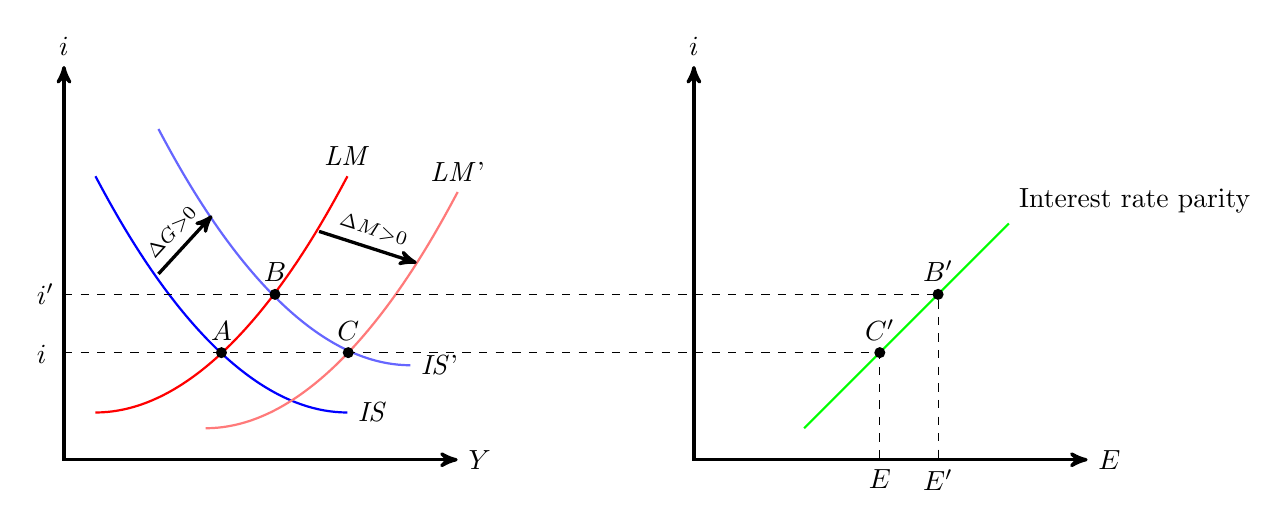
\begin{tikzpicture}[
        scale=2,
        IS/.style={blue, thick},
        LM/.style={red, thick},
        axis/.style={very thick, ->, >=stealth', line join=miter},
        important line/.style={thick}, dashed line/.style={dashed, thin},
        every node/.style={color=black},
        dot/.style={circle,fill=black,minimum size=4pt,inner sep=0pt,
            outer sep=-1pt},
    ]
    % axis
    \draw[axis,<->] (2.5,0) node(xline)[right] {$Y$} -|
                    (0,2.5) node(yline)[above] {$i$};
    % IS-LM diagram
    \draw[LM] (0.2,0.3) coordinate (LM_1) parabola (1.8,1.8)
        coordinate (LM_2) node[above] {\LM};
    \draw[IS] (0.2,1.8) coordinate (IS_1) parabola[bend at end]
         (1.8,.3) coordinate (IS_2) node[right] {\IS};
    %Intersection is calculated "manually" since Tikz does not offer
    %intersection calculation for parabolas
    \node[dot,label=above:$A$] at (1,.68) (int1) {};
    %shifted IS-LM diagram
    \draw[xshift=.7cm, LM, red!52] (0.2,0.2) parabola (1.8,1.7)
        node[above] {\LM'};
    \draw[xshift=.4cm, yshift=.3cm, IS, blue!60] (0.2,1.8)
        parabola[bend at end] (1.8,.3)
        node[right] {\IS'};
    %Intersection of shifted IS-LM
    \path[xshift=.36cm, yshift=.35cm] (.98,.7)
        node[dot,label=above:{$B$}] (int2) {};
    \path[xshift=.805cm] (1,.68) node[dot,label=above:$C$] (int3) {};
    %arrows between intersections
    \draw[->, very thick, black, >=stealth']
        ($(int1)+1/2*(-.80,1)$) -- ($(int2)+1/2*(-.8,1)$)
        node[sloped, above, midway] {$\mathsmaller{\Delta G > 0}$};
    \draw[->, very thick, black, >=stealth']
        ($(int2)+2*(.14,.2)$) -- ($(int2)!.2cm!270:(int2)+(.9,0)$)
        node[sloped,above, midway] {$\mathsmaller{\Delta M>0}$};
        
    \begin{scope}[xshift=4cm]
        %E-diagram
        \draw[axis,<->] (0,2.5) node(eyline)[above] {$i$} |-
                        (2.5,0) node(exline)[right] {$E$};

        \draw[important line, green, xshift=.5cm]
            (.2,.2) coordinate (es) -- (1.5,1.5) coordinate (ee)
            node [above right] {Interest rate parity};
    \end{scope}
    %Lines connecting IS LM coordinates and E coordinates
    \draw[dashed] 
        let
            % Store the intersection point in \p1 for later retrieval. 
            % A convenient feature of the let operation is that we can
            % access the x and y component of the coordinate directly 
            % using the \x1 and \y1 syntax. 
            \p1=(intersection of int2--[xshift=1]int2 and es--ee)
        in
            (0,\y1) node[left]{$i'$} -|  (\x1,0)
            node[pos=0.5,dot,label=above:$B'$] {} node[below] {$E'$};

    \draw[dashed line] let
        \p1=(intersection of int3--[xshift=1]int3 and es--ee)
            in
        (0,\y1) node[left]{$i\phantom{'}$} -| (\x1,0)
        node[dot,label=above:$C'$,pos=0.5] {} node[below] {$E$};

\end{tikzpicture}
\end{document}
%%% Local Variables:
%%% mode: latex
%%% TeX-master: t
%%% End: